\textbf{COLUNI 2024 -- Questão 33}\par\medskip Observe as informações sobre a população brasileira divulgadas no Censo Demográfico 2022, pelo Instituto Brasileiro de Geografia e Estatística - IBGE.

\begin{center}
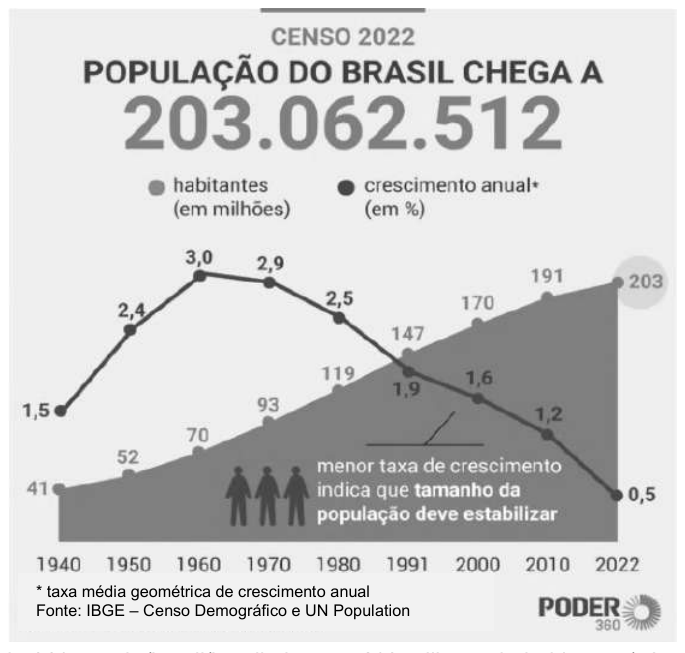
\includegraphics[width=0.52\linewidth]{static/simulados/coluni/figuras/2024/questao-33/figura-1.png}
\end{center}

Fonte: https://www.poder360.com.br/brasil/brasil-chega-a-203-milhoes-de-habitantes/. Acesso em: 5 ago. 2023.

De acordo com as informações contidas no gráfico e com os conhecimentos sobre demografia brasileira, observa-se que, a partir de 1960, a taxa média geométrica de crescimento anual da população diminui, enquanto a população absoluta continua aumentando. É CORRETO afirmar que o crescimento absoluto da população deve-se:
\begin{enumerate}
\item ao processo migratório elevado.
\item ao envelhecimento da população.
\item à piora nas condições de saúde e saneamento.
\item ao aumento da taxa de fertilidade.
\end{enumerate}
